
%-------------------------------LATEX SYNTAX----------------------------------
%
%       enter:                          \\, \linebreak, \newline
%       new page:                       \newpage
%       tab:                            \tab
%       new section:            \section{name} text
%       new paragraph           \subsection{name} text  (subsub...section{name} for more layers)
%       refer:                          \nameref{label name}    (place "\label{name}" at the position you want to refer to)
%       %, &, $, etc:           \%, \&, \$, etc         (these are latex operators, add a "\" to type it as text)
%       add comment:            \commred{text}, \commblue{text}, \commpurp{text}, \commgreen{text}
%       bullet points:          \begin{itemize} \item{text} ... \item{text} \end{itemize}
%       clean code:                     \cleancode{text}
%       idem without indent:\cleanstyle{text}
%       bold, italic, under:\textbf{text}, textit{text}, \underline{text}
%       table:                          \begin{tabular}{c c c} text \end{tabular}       ('&' for tab, '\\' for new line)
%       
%       use Google for the rest
%       
%------------------------------------------------------------------------------

\documentclass[a4paper]{report}

\usepackage[utf8]{inputenc}
\usepackage[english]{babel}
\usepackage{amsmath}
\usepackage{color}
\usepackage{graphicx}
\usepackage{grffile}
\usepackage{fancyref}
\usepackage{hyperref}
\usepackage{float}
\usepackage{scrextend}
\usepackage{setspace}
\usepackage{xargs}
\usepackage{multicol}
\usepackage{nameref}
\usepackage[pdftex,dvipsnames]{xcolor}
\usepackage{sectsty}
\usepackage{enumitem}
\usepackage{geometry}
\usepackage{listings}
\geometry{
 a4paper,
 total={170mm,257mm},
 left=20mm,
 top=20mm,
}

\graphicspath{ {images/} }
\newcommand\tab[1][1cm]{\hspace*{#1}}
\hypersetup{colorlinks=true, linkcolor=black}
\interfootnotelinepenalty=10000

\subsubsectionfont{\large}
\subsectionfont{\Large}
\sectionfont{\LARGE}

\definecolor{dkgreen}{rgb}{0,0.6,0}
\definecolor{gray}{rgb}{0.5,0.5,0.5}
\definecolor{mauve}{rgb}{0.58,0,0.82}

\lstset{frame=tb,
  language=bash,
  aboveskip=3mm,
  belowskip=3mm,
  showstringspaces=false,
  columns=flexible,
  basicstyle={\small\ttfamily},
  numbers=none,
  numberstyle=\tiny\color{gray},
  keywordstyle=\color{blue},
  commentstyle=\color{dkgreen},
  stringstyle=\color{mauve},
  breaklines=true,
  breakatwhitespace=true,
  tabsize=3
}


\definecolor{cleanOrange}{HTML}{D14D00}
\definecolor{cleanYellow}{HTML}{FFFF99}
\definecolor{cleanBlue}{HTML}{3d0099}

\newcommand{\cleanstyle}[1]{\text{\textcolor{cleanOrange}{\texttt{#1}}}}

\makeatletter
\providecommand*{\toclevel@lstlisting}{0}
\makeatother

\usepackage[colorinlistoftodos,prependcaption,textsize=footnotesize]{todonotes}
\newcommandx{\commred}[2][1=]{\textcolor{Red}
{\todo[linecolor=red,backgroundcolor=red!25,bordercolor=red,#1]{#2}}}
\newcommandx{\commblue}[2][1=]{\textcolor{Blue}
{\todo[linecolor=blue,backgroundcolor=blue!25,bordercolor=blue,#1]{#2}}}
\newcommandx{\commgreen}[2][1=]{\textcolor{OliveGreen}{\todo[linecolor=OliveGreen,
    backgroundcolor=OliveGreen!25,bordercolor=OliveGreen,#1]{#2}}}
\newcommandx{\commpurp}[2][1=]{\textcolor{Plum}{\todo[linecolor=Plum,
    backgroundcolor=Plum!25,bordercolor=Plum,#1]{#2}}}


%------------------------------------BEGIN DOC----------------------------------------

\begin{document}

\title{WAGASCI SOFTWARE\\INSTALLATION and USER GUIDE}
\author{\\Author: Pintaudi Giorgio\\\\
  Physics Department, Yokohama National University\\
  240-8501 Yokohama-shi Hodogaya-ku Tokiwadai 79-5\\ % chktex-file 8
  Minamino Laboratory\\
  Email: giorgio-pintaudi-kx@ynu.jp\\
  Phone: (+81) 070-4122-3907\\} \date{\today}
\maketitle
\newpage

% -----------------------------------------TOC-----------------------------------------
\tableofcontents\label{c}
\newpage

% ------------------------------------------TEXT---------------------------------------

\chapter{NEUT 5.4.0}
NEUT is a neutrino interaction simulation program library that has
been developed for the studies of the atmospheric neutrino and the
accelerator neutrinos. In this guide it is described how to compile
NEUT on a Linux machine. \textbf{NEUT 5.4.0} is the latest NEUT
version at the time of writing (\today). The author of this guide is
not the NEUT author, but it is a member of the T2K collaboration. NEUT
is not an open-source software and its sources \textbf{can be accessed
  only by T2K collaborators} in possession of a username and password
for the \href{https://www.t2k.org/}{T2K intranet}.

A fresh Linux installation is assumed, so, before compiling NEUT, I am
showing how to install or compile all NEUT dependencies. If you
already have some of the dependencies installed, you can safely skip
the relative paragraphs. Regarding the style of this guide, I wanted
to stay on the safe side so I have explained every step in
detail. This means that the guide could appear boring and
over-repetitive to a reader well-versed in Linux software compilation
and programming and I preventively apologize for that.

\section{List of NEUT dependencies}\label{dep}
To compile NEUT, three main dependencies are needed:
\begin{itemize}
\item \hyperref[]{\textbf{CERNLIB 2005}}\\
  CERNLIB 2005 is a quite old version of \cleanstyle{cernlib}, its
  latest release being dated 2012. Unsurprisingly it is quite tricky
  to compile. This is why I have included in the present guide a
  complete and detailed walk-through to the compilation of CERNLIB
  2005. There are several patches that need to be applied to both
  CERNLIB and NEUT source codes. Some of them were written by me, some
  others by Hayato-san.
\item \hyperref[root5]{\textbf{ROOT 5}}\\
  NEUT is compatible \textbf{only with ROOT 5} and not ROOT 6
  yet. There are plans to upgrade NEUT so to make it compatible with
  ROOT 6, but I don't know if there is any progress in that direction
  nor if there is any ETA.\ This plan was announced in the last T2K
  meeting in May. The latest and most updated version of ROOT 5 is
  \href{https://github.com/root-project/root/tree/v5-34-00-patches?files=1}{ROOT
    5.34.00-patches} (it is based on ROOT 5.34.39 and the latest
  commit on the that
  \href{https://github.com/root-project/root/tree/v5-34-00-patches?files=1}{GitHub
    branch} is March 2018) and I have chosen that for my personal
  installation.
\item \hyperref[]{\textbf{Fortran compilers}} (\cleanstyle{gfortran}
  and
  \cleanstyle{g77})\\
  The old fortran compiler \cleanstyle{g77} is not maintained anymore
  and, for example, it is not present in the Ubuntu repositories since
  the Ubuntu 8.04 Hardy Heron (my first Ubuntu, what
  nostalgia). Anyway, it is still possible to install it in a somewhat
  nonstandard way as it will be shown in the following.
\end{itemize}

\section{NEUT compatibility}
NEUT officially supports only CentOS 7, but this doesn't mean that it
cannot be run without issues on other Linux OSes. I will introduce
here 3 OSes that I have successfully compiled NEUT onto: CentOS 7,
Ubuntu 17.10 and Ubuntu 18.04. I will show how to compile NEUT only on
Ubuntu 18.04 64 bit because that is the most delicate case and because
Ubuntu 18.04 is the latest Ubuntu LST (Long Term Support) release.
\subsection{CentOS 7 - TO DO}
In May 2018 Hayato Yoshinari-san, who I think is also the main
developer of \href{https://inspirehep.net/record/844435?ln=en}{NEUT},
organized a small course about NEUT.\ Since the course was in Japanese
and I am not fluent yet, I could understand very little. Anyway, in
that occasion Hayato-san provided us with a CentOS 7 virtual machine
containing all the needed dependencies to compile and run NEUT.\ The
virtual machine can be downloaded from
\href{https://tinyurl.com/y8hy9kyr}{here}. I am not sure that this
link is of public dominion, but as far as it is circulated inside the
T2K collaboration there shouldn't be any problem.  The CentOS
virtual machine can be run through Oracle
\href{http://www.oracle.com/technetwork/server-storage/%
  virtualbox/downloads/index.html}{VM VirtualBox}.  The CentOS virtual
machine comes without any desktop manager. But it is possible to
install it if needed (I have installed GNOME). The user-name is
\cleanstyle{neut} and the password is \cleanstyle{neut5.4.0}. Here
some relevant details about it:
\begin{center}
  \begin{tabular}{||c | c||} % chktex-file 44
    \hline % chktex-file 44
    OS & CentOS 7 \\ [0.5ex] 
    \hline\hline % chktex-file 44
    kernel & 3.10.0-693.21.1.el7.x86\_64 \\
    \hline % chktex-file 44
    gcc/g++/gfortran & 4.8.5 20150623 (Red Hat 4.8.5-16) \\ 
    \hline % chktex-file 44
    ROOT & 5.28.00h+\\
    \hline % chktex-file 44
    CERNLIB & 2005 (dated 2016/12/12) \\
    \hline % chktex-file 44
    NEUT & 5.4.0 \\ [1ex] 
    \hline
  \end{tabular}
\end{center}

\subsection{Ubuntu 18.04}
With the aim of writing the present guide, I wanted to test
the NEUT compilation on a fresh install. I have chosen Ubuntu 18.04
because it is the latest Ubuntu LTS version, so in the following I
will assume an Ubuntu 18.04 64 bit fresh install.  Every other Linux
distribution should be compatible after minimal modification to some
of the shell commands, particularly regarding the package manager and
the package names. Notice that I haven't used the default Ubuntu 18.04
compiler (version 7.3.0) but I have installed the old 4.8 version of
\cleanstyle{gcc}, \cleanstyle{g++} and \cleanstyle{gfortran} as shown
in subsection~\ref{compiler}. 
\begin{center}
  \begin{tabular}{||c | c||} % chktex-file 44
    \hline % chktex-file 44
    OS & Ubuntu 18.04 \\ [0.5ex] 
    \hline\hline % chktex-file 44
    kernel & 4.15.0-23-generic \\ 
    \hline % chktex-file 44
    gcc/g++/gfortran & (Ubuntu 4.8.5-4ubuntu8) 4.8.5 \\
    \hline % chktex-file 44
    ROOT & 5.34.00-patches (patched version of ROOT 5.34.39) \\
    \hline % chktex-file 44
    CERNLIB & 2005 (dated 2016/12/12) \\
    \hline % chktex-file 44
    NEUT & 5.4.0 \\ [1ex] 
    \hline
  \end{tabular}
\end{center}

\section{Compile NEUT and its dependencies}
\subsection{Preliminaries}
\begin{enumerate}
\item Open a terminal or a shell. Ideally you should never close this
  shell from now until last step. If you need to close it nothing bad
  will happen but you might need to set up CERNLIB and ROOT
  environments again and/or come back to the right folder depending at
  which step you want to resume compilation.
\item\label{packages} First, we need to install some packages from the Ubuntu
  repositories. Some of them may be optional but I didn't have the
  patience to cherry-pick them. I have included them all just to be on
  the safe side. Do notice that it may take some time and space
  ($\sim$500MB).
\begin{lstlisting}
      sudo apt-get update && sudo apt-get upgrade
      sudo apt-get install build-essential git dpkg-dev cmake xutils-dev \
      g++ gcc gfortran binutils libx11-dev libxpm-dev libxft-dev libxext-dev \
      libssl-dev libpcre3-dev libglu1-mesa-dev libglew-dev \
      libmysqlclient-dev libfftw3-dev libcfitsio-dev libgraphviz-dev \
      libavahi-compat-libdnssd-dev libldap2-dev python-dev libxml2-dev \
      libkrb5-dev libgsl-dev libqt4-dev libmotif-dev libmotif-common \
      libblas-dev liblapack-dev csh tcsh gcc-4.8 g++-4.8 gfortran-4.8
\end{lstlisting}
\end{enumerate}

\subsection{Compilers}\label{compiler}
If you try to compile NEUT with compilers newer that 4.8, everything
will still compile fine but you will get the
following error on NEUT execution time:
\begin{lstlisting}
      !!!!!!!!!!!!!!!!!!!!!!!!!!!!!!!!!!!!!!!!!!!!!!!!!!!!!!!!!!!!
      LOCB/LOCF: address 0x7f68e28cd740 exceeds the 32 bit address space
      or is not in the data segments
      This may result in program crash or incorrect results
      Therefore we will stop here
      !!!!!!!!!!!!!!!!!!!!!!!!!!!!!!!!!!!!!!!!!!!!!!!!!!!!!!!!!!!!
\end{lstlisting}
This error is ultimately connected to the \cleanstyle{FFKEY} call in
fortran. \cleanstyle{FFKEY} allows something which is read in to 
be an integer or float at a later time in the run. This should not 
be allowed (and isn't) by modern standards, but is still in CERNLIB
and NEUT.\@ 

To switch between compilers, create and make executable the following
shell script
\begin{lstlisting}
      #!/bin/sh

      if [ -z "$1" ]; then
          echo "usage: $0 version" 1>&2
          exit 1
      fi

      if [ ! -f "/usr/bin/gcc-$1" ] || [ ! -f "/usr/bin/g++-$1" ] || [ ! -f "/usr/bin/gfortran-$1" ]; then
          echo "no such version gcc/g++/gfortran installed" 1>&2
          exit 1
      fi

      sudo update-alternatives --set gcc "/usr/bin/gcc-$1"
      sudo update-alternatives --set g++ "/usr/bin/g++-$1"
      sudo update-alternatives --set gfortran "/usr/bin/gfortran-$1"
\end{lstlisting}
The script accepts as the only and compulsory parameter the version of
the compiler to switch into. It is \cleanstyle{4.8} for 4.8 compilers
and \cleanstyle{7} for the 7.x compilers.

Be sure to run the script and switch to the 4.8 compiler before
starting the compilation of ROOT, CERNLIB and NEUT.\@ 

\subsection{ROOT 5}\label{root5}
As already pointed out in the introduction, at the time of writing,
\textbf{NEUT 5.4.0 is only compatible with ROOT 5}. Please refer to
section~\ref{dep} for further details about this ``issue''.  Here I
will explain how to compile ROOT 5.34.00-patches starting from the
source code since it is the safest way to insure that everything is
functioning correctly: if there is any incompatibility it is usually
reported at compilation time, while, if you install ROOT through the
pre-compiled binaries, any incompatibility will be uncovered only at
run time, when the errors can be more obscure and misleading to
interpret.

I recommend the use of the ``three folders'' procedure to install
ROOT.\ One folder is for the source code, one for the
compiling/building and one for the final installation. The sources
folder is managed entirely using git and it contains a copy of the
ROOT git repository. You can checkout the branch that you need to
compile at any time. Another folder contains the temporary building
files (such as the object files). It is effectively used only during
compilation and can be removed afterwards. It is quite heavy (about
3GB) so I usually delete it as soon as I have installed ROOT.\@ The
last folder is the installation folder where a certain version of ROOT
is installed. When running ROOT, in fact only this folder is needed.

I am showing now how to install ROOT.\@ The following instructions are
freely taken from the following pages:
\begin{itemize}
\item \href{https://root.cern.ch/building-root}{Building root}
\item
  \href{https://d35c7d8c.web.cern.ch/root-version-v5-34-00-patch-release-notes}%
  {ROOT v5-34-00-patch release-notes}
\item \href{https://root.cern.ch/build-prerequisites}{Build
    prerequisites}
\end{itemize}

\begin{enumerate}[resume]
\item Open a terminal if not already opened.
\item\label{root-1} Then install some fonts required by ROOT%
\begin{lstlisting}
      sudo apt install xfstt xfsprogs t1-xfree86-nonfree ttf-xfree86-nonfree \
      ttf-xfree86-nonfree-syriac xfonts-75dpi xfonts-100dpi
\end{lstlisting}
  You can optionally install the following packets to have a more
  thorough ROOT installation. They are by no means mandatory. I
  honestly have no idea what many of these packages do. I just hate
  dealing with missing dependencies when I run software.
\begin{lstlisting}
      sudo apt install libgif-dev libtiff-dev libjpeg-dev liblz4-dev \
      liblzma-dev libgl2ps-dev libpostgresql-ocaml-dev libsqlite3-dev \
      libpythia8-dev davix-dev srm-ifce-dev libtbb-dev python-numpy
\end{lstlisting}
  
\item\label{root-2} Create two directories that will contain the ROOT source code
  and the compiled code. You can change the paths as you wish, but
  then you have to remember to change all the references and links in
  the following accordingly. You may also need to modify the patches
  since they include these paths.
\begin{lstlisting}
      mkdir -p $HOME/Code/ROOT/{sources,5-34-00-patches,5-34-00-patches-build}
      cd $HOME/Code/ROOT
\end{lstlisting}
\item\label{root-3} Clone the ROOT source code into the sources directory using git
  and then:
\begin{lstlisting}
      git clone http://github.com/root-project/root.git sources
      cd sources
      git checkout -b v5-34-00-patches origin/v5-34-00-patches
      cd ../5-34-00-patches-build
\end{lstlisting}
\item\label{root-4} Execute the cmake command on the shell.
\begin{lstlisting}
      cmake -Dbuiltin_xrootd=ON -DCMAKE_INSTALL_PREFIX=$HOME/Code/ROOT/5-34-00-patches ../sources
\end{lstlisting}
  CMake will detect your development environment, perform a series of
  test and generate the files required for building ROOT.\@
\item After CMake has finished running, start the build from the build
  directory:
\begin{lstlisting}
      cmake --build . --target install
\end{lstlisting}
  On UNIX systems (with make or ninja) you can speedup the build with%
\begin{lstlisting}
      cmake --build . --target install -- -jN
\end{lstlisting}
  where N is the number of available cores.
\item Now you can safely remove the build directory if you need that
  space.
\begin{lstlisting}
      cd
      rm -Rf $HOME/Code/ROOT/5-34-00-patches-build
\end{lstlisting}

\item Every time that you run ROOT, you need to setup the
  environment. There are at least three ways to do that, more ore less
  automated.
  \begin{itemize}
  \item One is to run the command%
\begin{lstlisting}
      source $HOME/Code/ROOT/5-34-00-patches/bin/thisroot.sh
\end{lstlisting}
    Every time it is needed.
  \item Another way is to define an alias in the
    \cleanstyle{.bash\_aliases} file or in the \cleanstyle{.bashrc}
    file. For instance I have set
\begin{lstlisting}
      alias root5='source $HOME/Code/ROOT/5-34-00-patches/bin/thisroot.sh'
      alias root6='source $HOME/Code/ROOT/6-12-06/bin/thisroot.sh'
\end{lstlisting}
    To quickly switch between different ROOT versions.
  \item Alternatively one can set up the correct root environment at
    boot by inserting the following lines in the \cleanstyle{.profile}
    file
\begin{lstlisting}
      # set the needed environment variables, PATH and LD_LIBRARY_PATH for root
      if [ -f "${HOME}/Code/ROOT/5-34-00-patches/bin/thisroot.sh" ] ; then
      source ${HOME}/Code/ROOT/5-34-00-patches/bin/thisroot.sh
      fi
\end{lstlisting}
    Then every shell will have that version of root as default.
  \end{itemize}
\item Before using root, remember to reboot (to reload the
  fonts). Then you can ROOT with the command \cleanstyle{root}.
\end{enumerate}

\subsection{CERNLIB 2005}
The following procedure was freely taken from the three reference web
pages:
\begin{itemize}
\item
  \href{https://www.t2k.org/asg/xsec/niwgdocs/neut/install_neut}{NEUT
    installation}
\item
  \href{https://www-zeuthen.desy.de/linear_collider/cernlib/new/cernlib_2005.html}%
  {CERNLIB installation }
\item
  \href{http://seanelvidge.com/2017/01/install-g77-on-ubuntu-14-04/}{g77
    installation}
\end{itemize}
\begin{enumerate}[resume]
\item Create a new folder for CERNLIB and move to it. In the following
  I am assuming that you won't leave that folder until the CERNLIB
  compilation is complete.
\begin{lstlisting}
      mkdir $HOME/Code/CERNLIB
      cd $HOME/Code/CERNLIB
\end{lstlisting}
\item CERNLIB uses a different naming for make. I suppose this is due
  to small differences in naming conventions between UNIX and Linux
  (g-nu).%
\begin{lstlisting}
      sudo ln -s /usr/bin/make /usr/bin/gmake
\end{lstlisting}
\item The following commands add the hardy repositories to the
  \cleanstyle{sources.list} file and install \cleanstyle{g77}. This
  step is needed to download and install the fortran \cleanstyle{g77}
  compiler. It is advisable to comment or remove these lines after the
  \cleanstyle{g77} installation.%
\begin{lstlisting}
      sudo tee -a /etc/apt/sources.list << END

      # Old hardy repository needed to install g77
      # It is recommended to comment or remove following lines after g77 installation
      
      deb [trusted=yes] http://old-releases.ubuntu.com/ubuntu/ hardy universe
      deb-src [trusted=yes] http://old-releases.ubuntu.com/ubuntu/ hardy universe
      deb [trusted=yes] http://old-releases.ubuntu.com/ubuntu/ hardy-updates universe
      deb-src [trusted=yes] http://old-releases.ubuntu.com/ubuntu/ hardy-updates universe
      END
      sudo apt-get update && sudo apt-get install g77
\end{lstlisting}
\item Now it is time to solve a couple of bugs of the \cleanstyle{g77}
  compiler. This is quite an old and now largely obsolete
  compiler. For this reason many adjustments are needed to get it
  working. You may need to modify the code below if your system libraries
  path or your gcc compiler version are different. For more
  information and troubleshooting please consider visiting
  \href{http://seanelvidge.com/2017/01/install-g77-on-ubuntu-14-04/}{this
    page}.

  The following command will create a symbolic link of a library that
  \cleanstyle{g77} would not able to find otherwise.
\begin{lstlisting}
      sudo ln -s /usr/lib/gcc/x86_64-linux-gnu/7/libgcc_s.so /usr/lib/x86_64-linux-gnu/
\end{lstlisting}
\item  Then let us set up the \cleanstyle{LIBRARY\_PATH} environment
  variable. This must be done every time you want to use the
  \cleanstyle{g77} compiler.
\begin{lstlisting}
      export LIBRARY_PATH="/usr/lib/x86_64-linux-gnu:\$LIBRARY_PATH"
\end{lstlisting}
If you want to avoid issuing the previous command every time, you can
do the following:
\begin{lstlisting}
      tee -a $HOME/.profile << END

      # set LIBRARY_PATH so it includes x86_64-linux-gnu if it exists
      if [ -d "/usr/lib/x86_64-linux-gnu" ] ; then
      LIBRARY_PATH="/usr/lib/x86_64-linux-gnu:\$LIBRARY_PATH"
      export LIBRARY_PATH
      fi
      END
\end{lstlisting}
  
\item Download all the CERNLIB 2005 source code archives:%
\begin{lstlisting}
wget http://www-zeuthen.desy.de/linear_collider/cernlib/new/cernlib-2005-all-new.tgz
\end{lstlisting}
 \begin{lstlisting} 
wget http://www-zeuthen.desy.de/linear_collider/cernlib/new/cernlib.2005.corr.2014.04.17.tgz
\end{lstlisting}
\begin{lstlisting}
wget http://www-zeuthen.desy.de/linear_collider/cernlib/new/cernlib.2005.install.2014.04.17.tgz
\end{lstlisting}
\item Extract the downloaded files:
\begin{lstlisting}
      tar -zxvf cernlib-2005-all-new.tgz
      cp cernlib.2005.corr.2014.04.17.tgz cernlib.2005.corr.tgz
      tar -zxvf cernlib.2005.install.2014.04.17.tgz
\end{lstlisting}

\item Download my patched version of the old \cleanstyle{patchy 4}
  source code and substitute it with the non patched one. I am not
  sure if the \cleanstyle{patchy} suite is really necessary for NEUT
  but it is better to have and not need it than need it and not have.
\begin{lstlisting}
rm patchy4.tar.gz
wget https://www.dropbox.com/s/n7n1wiivn1noets/patchy4.tar.gz
\end{lstlisting}

  
\item Download and check the patch:
\begin{lstlisting}
      wget https://www.dropbox.com/s/loa53mklvotzsvj/jojo-CERNLIB.patch
      cp Install_cernlib Install_cernlib.backup
      patch -p0 --dry-run < jojo-CERNLIB.patch
\end{lstlisting}
\item If there isn’t any error, patch the installation script
\begin{lstlisting}
      patch -p0 < jojo-CERNLIB.patch
\end{lstlisting}
\item Now you can compile CERNLIB.\@ 
\begin{lstlisting}
      ./Install_cernlib
\end{lstlisting}
\item Check that the compilation process went well by looking for
  errors in the log files in \cleanstyle{2005/build/log}
  \begin{lstlisting}
      grep ./2005/build/log -R -i -e "error [0-9]" | grep -v ZDROP | grep -v ZBOOKN
\end{lstlisting}
\item Finally set up the CERNLIB environment for the next section.
\begin{lstlisting}
      source cernlib_env
\end{lstlisting}
\end{enumerate}

\section{NEUT 5.4.0}
\begin{enumerate}[resume]
\item If you are continuing from the same terminal as the previous
  section, you don't need this step. Otherwise open the terminal and
  issue the following commands to setup the NEUT compilation
  environment:
\begin{lstlisting}
      source $HOME/Code/ROOT/5-34-00-patches/bin/thisroot.sh
      source $HOME/Code/CERNLIB/cernlib_env
\end{lstlisting}
\item Create the NEUT folder and move to it.
\begin{lstlisting}
      mkdir $HOME/Code/NEUT
      cd $HOME/Code/NEUT
      export NEUT_ROOT=$HOME/Code/NEUT
\end{lstlisting}
\item Download the NEUT source code from
  \href{https://www.t2k.org/asg/xsec/niwgdocs/neut/NEUT5.4.0}{this
    link}. To download the file it is necessary to insert one's own
  T2K credentials. Then move the downloaded archive in the NEUT
  folder. During the download don't close the terminal. Go back to the
  terminal and issue: 
\begin{lstlisting}
      cd $HOME/Code/NEUT
      mv neut_5.4.0_20180120.tar.gz neut_5.4.0_20180120.tar
      tar -xvf neut_5.4.0_20180120.tar
      mv neut_5.4.0/src ./src
      rmdir neut_5.4.0
\end{lstlisting}
\item Download and check the patches
\begin{lstlisting}
      cd src/neutsmpl
      wget https://www.dropbox.com/s/dxyjk5fzw0vuv85/jojo-NEUT-1.patch
      wget https://www.dropbox.com/s/ew07kn9duzvhqtt/jojo-NEUT-2.patch
      patch -p0 --dry-run < jojo-NEUT-1.patch
      patch -p0 --dry-run < jojo-NEUT-2.patch
\end{lstlisting}
\item If there aren't errors, apply the patches:
\begin{lstlisting}
      patch -p0 < jojo-NEUT-1.patch
      patch -p0 < jojo-NEUT-2.patch
\end{lstlisting}
\item Finally compile NEUT.\@ All should be fine now.
\begin{lstlisting}
      ./Makeneutsmpl.csh
\end{lstlisting}
\end{enumerate}

\chapter{ROOT 6}
ROOT is a modular scientific software framework. It provides all the
functionalities needed to deal with big data processing, statistical
analysis, visualization and storage. It is mainly written in C++ but
integrated with other languages such as Python and R\footnote{Text
  taken from ROOT homepage}.

This chapter is very short because much of the content that should go
here is already covered in section~\ref{root5}. The only real
difference is that here we are compiling the latest version of ROOT with
the latest compilers (at the time of writing: \today).

I am assuming here that you have never installed ROOT before. That is
why we are cloning the git repository. If you already have another
installation of ROOT and you just want to upgrade or reinstall, please
make the proper modification to these steps. I am assuming that you
are capable of that.

This chapter is tailored towards Ubuntu 18.04 but it should be the
same for any other Linux distribution with some minor modifications.

\section{Preliminaries} First install all the packages listed in
section~\ref{packages}. Again, some of them may not be strictly needed
but cherry-picking which package is needed and which not could be very
time consuming. If you have very strict space limitations and you are
somewhat forced to install the least amount of software, I really feel
sorry for you but don't expect me to willingly help you\dots

Then make you sure you are using the last version of the compilers by
issuing
\begin{lstlisting}
      gcc --version
\end{lstlisting}
The output should be
\begin{lstlisting}
      gcc (Ubuntu 7.3.0-16ubuntu3) 7.3.0
      [...]
\end{lstlisting}

\section{ROOT Installation}

Then follow the step~\ref{root-1} of section~\ref{root5}. Instead of step~\ref{root-2}, type
\begin{lstlisting}
      mkdir -p $HOME/Code/ROOT/{sources,6-14-02,6-14-02-build}
      cd $HOME/Code/ROOT
\end{lstlisting}
Instead of step~\ref{root-3}, type
\begin{lstlisting}
      git clone http://github.com/root-project/root.git sources
      cd sources
      git checkout -b v6-14-02 v6-14-02
      cd ../6-14-02-build
\end{lstlisting}
Instead of step~\ref{root-4}, type
\begin{lstlisting}
      cmake -Dbuiltin_xrootd=ON
-DCMAKE_INSTALL_PREFIX=$HOME/Code/ROOT/6-14-02 ../sources
\end{lstlisting}

The following steps are the very same of section~\ref{root5} where in
place of \cleanstyle{5-34-00-patches} you just have to type
\cleanstyle{6-14-02}.

\chapter{DAQ software}
The main software for data acquisition of the WAGASCI experiment is
called Anpan (Acquisition Networked Program for Accelerated
Neutrinos). It is based on the Calicoes software that was used for the
Silicium Tungsten Electromagnetic Calorimeter (SiW-ECAL) prototype of
the future International Linear Collider, developed by Frédéric
Magniette and Miguel Rubio-Roy. Both Anpan and Calicoes are based on
the Pyrame framework of which they two similar implementations.

Until Summer 2018, we were using the Calicoes software without almost
any modification as the data acquisition software for the WAGASCI
prototype (i.e. Proton Module + WAGASCI water-in detector + Ingrid
module).

Between the end of the WAGASCI prototype commissioning run in Summer
2018 and the beginning of the WAGASCI Experiment Physics run in April
2019, I started my Ph.D. at YNU and I decided to further develop and
improve the WAGASCI DAQ system. So I took the decision (quite
one-sidedly I have to admit) to change the name of the acquisition
software and release it under the GPLv3 license.

It is not clear which license is Calicoes released according
to. Anyway Pyrame (which is written by the same developers) is
released under GPLv3 so I assumed that Calicoes is released under the
same license. This entitles me (Pintaudi Giorgio) to release again a
modified version of the software under different name but giving due
credit to the original authors (Frédéric Magniette and Miguel
Rubio-Roy).

I have chosen that name because wagashi (after which the WAGASCI
experiment is named) in Japanese means ``traditional sweets'' and
anpan (a soft bun filled with red soy beans paste) is a kind of
Japanese sweet snack (even if not properly an strictly traditional
sweet). Anyway, I love anpan and I eat one of them almost everyday so
we can say that the development of this software was fueled mainly by
anpan. From that the name choice.

This chapter of the documentation isn't a thorough guide of all the
code that makes up anpan because much of that is already explained in
the \href{http://llr.in2p3.fr/sites/pyrame/documentation/}{Pyrame
  documentation website} and
\href{http://llr.in2p3.fr/sites/pyrame/calicoes/documentation/}{Calicoes
  documentation website}. Anyways those websites are mainly aimed at
developers who are well-versed in scientific programming and are not
afraid of reading through much of the source code. Instead, this guide
is meant to be a user manual for the physicist who just wants to use
the software (and maybe only write some simple scripts).

One must always keep in mind that most of the times scientific
software is not written by a big team of programmers with a steady job
and a steady income, but by a few researchers or worse grad students
with little (or no) income whatsoever, unsteady future prospects and a
very limited budget. Because of the lack of money and man-power,
usually the first thing that get cut or reduced is documentation
(because it is not strictly necessary for the software to run). This,
as long as the original developers are also the users of the software,
has no tangible consequences. But as new physicists start to use the
software an evil-loop onsets where software is used just as-is and
works-just-because-it-works. Luckily the Calicoes and Pyrame software
is adequately documented and with this guide I would like to close the
gap between users and software even further.

\section{Pyrame}
I won't go into detail describing the Pyrame framework since much of
what I have to say is already covered in the
\href{http://llr.in2p3.fr/sites/pyrame/documentation/}{Pyrame
  documentation website}. So before continuing to the following I
would suggest the reader to take a quick look there and get a rough
idea of what is happening inside of Pyrame. This section is merely
intended as an appendix and a review of the content shown there. The
only real difference with the online documentation is that, instead of
trying to explain how the software works, I will take the point of
view of the user and I will only focus on how to use Pyrame to get
some work done.

First, what the user need to understand is that Pyrame is a
distributed software. This means that each part or function of Pyrame
can be located on a different machine. Each of those parts are called
``modules'' and each module communicates with the others through the
exchange of TCP/IP packets. If you don't know what the TCP/IP protocol
is you can consult the Wikipedia pages:
\href{https://en.wikipedia.org/wiki/Transmission_Control_Protocol}{TCP}
and \href{https://en.wikipedia.org/wiki/IPv4}{IP}, that should be
enough.

Basically each machine able to get an IP address can open a network
port through which a certain application (or in the case of Pyrame a
certain module) can communicate and interact with the modules
``outside''. For modules residing on the same machine the
\cleanstyle{localhost=127.0.0.1} IP address must be used. The purpose
of the localhost IP address is simply to send an outgoing packet back
in. So for example if we want to reach the Configuration Module (CMOD)
that is running on the port \cleanstyle{CMOD\_PORT=9002} on the local
machine we need the only to use the couple
\cleanstyle{localhost:CMOD\_PORT} or explicitly
\cleanstyle{127.0.0.1:9002}. Or if we want to communicate with the
Variables Module (VARMOD) that is running on the port
\cleanstyle{VARMOD\_PORT=9001} on another machine in the same sub-net
with IP \cleanstyle{192.168.10.100} we would address it as
\cleanstyle{192.168.10.100:9001} and so on.  The list of all the
default ports is located in \cleanstyle{/opt/pyrame/ports.txt}

There are 7 fundamental modules that must be always running during
data acquisition for Pyrame to function correctly:
\begin{itemize}
\item The Variables module: \cleanstyle{VARMOD\_PORT=9001}
\item The Configuration module: \cleanstyle{CMOD\_PORT=9002}
\item The Mount Datadir Module: \cleanstyle{MOUNTD\_PORT=9005}
\item The Acquisition-Chain Module: \cleanstyle{ACQ\_PORT=9010}
\item The Run Control Module: \cleanstyle{RC\_PORT=9014}
\item The Storage Module: \cleanstyle{STORAGE\_PORT=9020}
\end{itemize}
There may be other modules running depending on the specific
configuration. The needed modules are usually started automatically
when a configuration file is loaded so the user doesn't need to worry
about that. To learn more about the configuration file go to section
TO-DO.

Starting from Section~\ref{sec:CMOD} I will give a short description
of each of these modules, but before that I would like to talk about
the ``State Machine''.

\subsection{State Machine}
In Pyrame, the detector is always thought to be in one of four
states. They are:
\begin{enumerate}
\item\label{undefined} UNDEFINED: The detector state has not been
  probed yet. This is the state of the detector before Pyrame has
  started or after it has ended.
\item READY: The detector itself is in the same UNDEFINED state as
  before but the software has been initialized and the detector
  configuration has been loaded into memory.
\item CONFIGURED or RECONFIGURED: The configuration has been applied
  to the detector. This means that the firmware of the various boards
  has been configured, the power supplies turned on, the voltage set
  up and so on. The detector is ready to take data.
\item\label{acquiring} ACQUIRING The detector is acquiring data.
\end{enumerate}
The principle at the base of the Pyrame workflow is that the user must
go through all the steps from~\ref{undefined} to~\ref{acquiring} in
order to take data. The software will take charge of managing all the
synchronization issues.  All the transitions between machine state can
be accomplished with the aid of shell scripts called from a terminal:
\cleanstyle{load\_config\_file.sh}, \cleanstyle{initialize.sh},
\cleanstyle{configure.sh}, etc\dots. It is also possible to use the
CouchDB web-GUI to manage the transitions.
\begin{figure}
  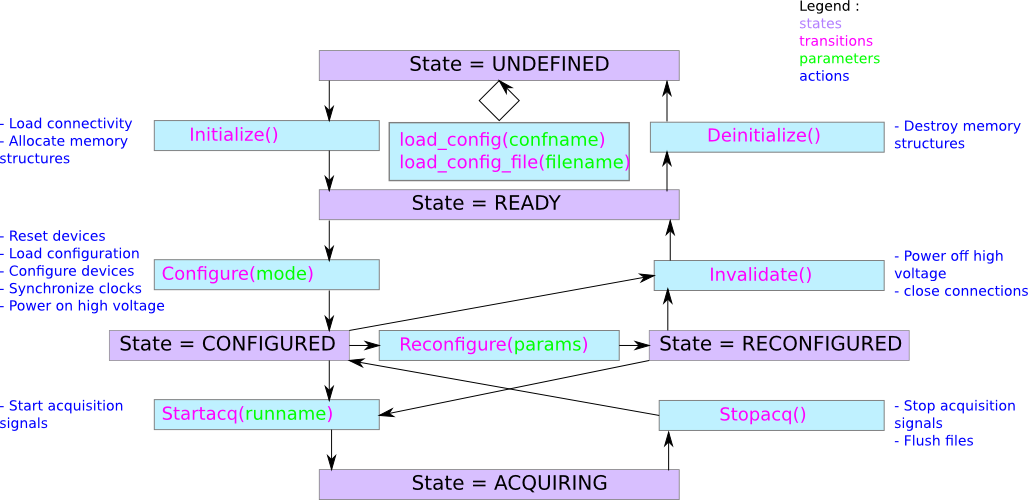
\includegraphics[width=\linewidth]{state_machine.doc.png}
  \caption{Pyrame State Machine}
  \label{fig:state-machine}
\end{figure}

\subsection{The Configuration Module}
\label{sec:CMOD}

The configuration module (called also CMOD) is in charge of many
things. First, it is dedicated to configuration storage and export.
Every Pyrame module can register in the cmod and store its
configuration parameters. The configuration parameters and the modules
themselves are organized as a tree-like structure representing the
actual structure of the detector.  TO-DO how modules can edit the
configuration?

Usually the user just load a configuration file in the cmod using the
shell script \cleanstyle{load\_config\_file.sh filename.xml}. The cmod
contains at any time a copy of the configuration of all the modules
and it can generate xml files containing all the parameters to be used
with calxml.

Another role that cmod plays is to manage the transitions between
different states through the \cleanstyle{transition\_cmod}
function. Again, usually this transition is managed by shell scripts
or directly by the GUI so cmod is quite transparent to the user.

\subsection{The Variables Module}
\label{sec:VARMOD}

The varmod is a centralized service that allows all the modules to
share variables for collecting statistics or sharing global
information. You can store a value associated with a name (a variable)
and then get it back. You can also make some basic operations on the
variables. For more information refer to the Pyrame documentation.

\subsection{The Acquisition-Chain Module}
\label{sec:ACQ}
In my opinion, understanding completely the Pyrame Acquisition-Chain
is the most daunting task, if one really wants to know how the Pyrame
software works internally. Since I am far from an expert in that
field, I will only gather here what I have understood so far.

From the perspective of the user, reading the
\href{file:///opt/pyrame/doc/cmd_acq.html}{Pyrame documentation}, the
comments in the configuration file and the comments in the
\cleanstyle{cmd\_acqpc.py} file should be enough to get things going
in almost every real-world scenario.

For the developers and more experienced users let's start by taking a
look at the graph~\ref{fig:acq-server}:
\begin{figure}
  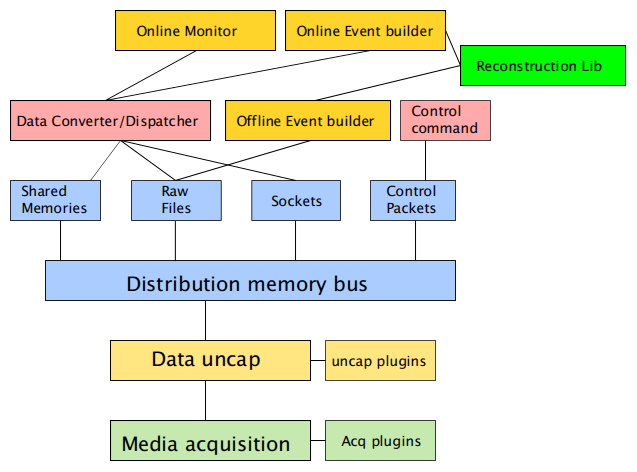
\includegraphics[width=\linewidth]{acq_server.doc.png}
  \caption{Pyrame State Machine}
  \label{fig:acq-server}
\end{figure}
I will only focus on the WAGASCI case. All the configuration regarding
the acquisition chain is done under the \cleanstyle{pcacq\_X} field in
the configuration file. If you take a pre-existing configuration file
written by myself you will find many descriptive comments in that
section that hopefully will guide you through a painless
configuration.

\subsubsection{Media acquisition}
The ``media acquisition'' phase is controlled by the acquisition
plugins. What these plugins do is to ``open'' an acquisition media and
get the data from there. The acquisition media can basically be of two
types: the Ethernet port (with TCP or UDP protocols) or a raw file
that was previously acquired (for testing or debugging purposes). For
a more in-depth description of every plugin refer to
\href{file:///opt/pyrame/doc/cmd_acq.html}{this page} and its
sub-pages. After the data has been acquired, it is not ready to be
analyzed yet because it contains the IP/TCP caps and it is in binary
form.

You can take a look at the source code and related comments in the
\cleanstyle{anpan/cmd\_acqpc/cmd\_acqpc.py} file and in particular in
the \cleanstyle{init\_fin\_acqpc} function where every acquisition
plugin is listed and explained.

\subsubsection{Data uncap}
In this face, the acquired data is uncapped. This means that, for
example in the TCP case, the IP/TCP headers are stripped, the data
integrity checked (lost or corrupted packages) and the data content
filtered (data packets or control packets). Honestly I don't know much
more than this about these plugins.

\subsubsection{Data Converter/Dispatcher}
Here the decoder library is called. For example in the case of
SPIROC2D the library path is \cleanstyle{spiroc2d\_decoder.so}. This
library takes the uncapped raw data coming from the acquisition source
(for example the GDCC) and convert it into a stream of blocks of
events. These blocks are then fed to the Online Monitor and Online
Event Builder programs.  The decoder library needs to know the channel
mapping (the geometry) of the detector to associate to every channel
its position in space.

However, maybe because of some bugs or lack of time, the SPIROC2D
converter for the WAGASCI prototype commissioning run was disabled. In
the \cleanstyle{cmd\_dif.py} file the line needed to start the
conversion was commented out and function's result was always set to
positive, thus completely disabling Online Monitor capabilities of
Pyrame.

I am going to enable it again and debug it (TO-DO)

\subsubsection{Online Monitor}
The WAGASCI online monitor code is contained in the
\cleanstyle{anpan/guis/om\_wagasci} folder. It is a program external
to Pyrame and WAGASCI that needs to be started by hand. It however
interacts with Pyrame under the hood. It receives the Blocks and
Events created by the ``Data Converter/Dispatcher'' face. More info
about the More info can be found in section TO-DO.

\subsection{The Run Control Module}
\label{sec:RC}

TO-DO

\subsection{The Storage Module}
\label{sec:STORAGE}

Storage is a Pyrame module that manages data created by other modules
and its inclusion on the RunDB. For further info about the RunDB
module refer to the Pyrame documentation.

Storage allows to use a mount point and a path to transparently store
data elsewhere in the network. It also automates common tasks such as
saving the calxml configuration and a log with optional varmod
variables (e.g.: stats) at the same place as data files.

As far as I know there are only two kinds of storage that the Storage
Module can handle. One is the standard file on a file system and
another one is a NFS share on the network.

In the case of a standard file this is the format for the mp variable:
\begin{lstlisting}
      <param name="storage_brg_mp">file:///</param>
\end{lstlisting}
In the case of a NFS share this is the format for the mp variable:
\begin{lstlisting}
      <param name="storage_brg_mp">nfs://server/nfs</param>
\end{lstlisting}

% To autostart services (modules) when Pyrame is started edit file
% pyrame/launcher/services.txt To add default module ports edit the
% file pyrame/ports.txt

\subsection{Run and interact with Pyrame}
There are several ways to interact with Pyrame and its modules. When
the AnpanInstaller script installs Pyrame, it makes sure that Pyrame
is automatically started at every reboot. On system with
\cleanstyle{systemctl}\footnote{Both Ubuntu 18.04 and CentOS 7 use
  \cleanstyle{systemctl}} Pyrame is started as a system daemon and its
execution is controller with the \cleanstyle{systemctl} or
\cleanstyle{service} shell commands. To enable Pyrame at startup use
\begin{lstlisting}
      sudo systemctl enable pyrame
\end{lstlisting}
To disable it
\begin{lstlisting}
      sudo systemctl disable pyrame
\end{lstlisting}
To start a single time Pyrame
\begin{lstlisting}
      sudo systemctl start pyrame
\end{lstlisting}
To stop it
\begin{lstlisting}
      sudo systemctl stop pyrame
\end{lstlisting}

Moreover there are several ways to interact with Pyrame modules. If a
module is already running the simplest way to interact with it is to
open a terminal and use the command:
\begin{lstlisting}
      chkpyr2.py hostname port function parameters
\end{lstlisting}
where \cleanstyle{hostname} is the IP address of the module, for
example \cleanstyle{localhost}, \cleanstyle{port} is the port number
of the module, \cleanstyle{function} is the particular function that
you want the module to perform and \cleanstyle{parameters} are the
parameters to be passed to that function. All the public functions of
the Pyrame and Anpan/Calicoes modules are listed on the online
documentations.

You can also interact with Pyrame modules from external python scripts
... TO-DO

\subsection{Pyrame Configuration}\label{sec:pyrame-configuration}
TO-DO

\subsection{Blocks and Events}\label{sec:blocks-events}
In Pyrame the raw data is organized in events and blocks of events. As
far as I understood, events are grouped into blocks that are sent
between Pyrame modules.

\subsubsection{Event}
On a raw level, an event is just a single hit TO-CHECK. Each hit is
roughly described by the time, space and charge released. Other
parameters that may refer to an event are described below.

An event is described by a struct like this:
\begin{lstlisting}
      struct event {
        char **time;             // List of string containing hit times
        int time_size;           // Number of hit times
        char **space;            // List of string containing hit points
        int space_size;          // Number of hit points
        char **data;             // List of string containing various
                                 // event properties.
        int data_size;           // Number of elements in data
        char used;               // ??
        struct event *next;      // Pointer to the next event
        struct block *block;     // Pointer to the block
      };
\end{lstlisting}
Up to now the \cleanstyle{data} list contains the following elements:
\begin{itemize}
\item ``spill'': spill number.
\item ``spill\_flag'': the spill flag is set when the event happens
  inside of the beam spill time-frame. This means that the particle
  detected is most probably the result of a neutrino interaction from
  the neutrino beam inside or outside the detector.
\item ``roc'': ROC chip number.
\item ``rocchan'': ROC chip channel number.
\item ``bcid'': BCID (Bunch Crossing IDentification). Despite the
  misleading name, the BCID indicates just the number of rise time of
  the slow since the \textit{startacq} signal. More on this on TO-DO.
\item ``sca'': Switched Capacitor Array number.
\item ``plane'': Plane number.
\item ``channel'': Channel number.
\item ``en'': Energy (charge). This field correspond to the ADC count.
\item TDC time: ``time''
\item ``hit'': The hit flag is set if the event contains a hit. The
  hit may be due to a particle passage inside of the detector or
  simply by dark or electric noise.
\item ``gain'': The gain flag is set when we want to measure the
  gain. In that case we compare the pedestal and first hit position to
  calculate the gain.
\end{itemize}

\subsubsection{Block}
A block is described by a struct like this:
\begin{lstlisting}
      struct block {
        int id;                  // Block identifier
        char finalized;          // ??
        int nb_events;           // Number of events in the block
        char **props;            // List of strings that can contain
                                 // various block properties as the
                                 // spill number, spill flag, etc...
        int props_size;          // Number of props strings
        char *bstr;              // ??
        struct evtstruct *es;    // This struct is used to navigate
                                 // through the various props strings
        struct event *events;    // List of events
        struct block *next;      // Pointer to the next block
      };
\end{lstlisting}
Up to now the \cleanstyle{props} list contains the following elements:
\begin{itemize}
\item spill number: ``spill''
\item spill flag: ``spill\_flag''
\end{itemize}

The ``spill\_flag'' is ``1'' during the spill time frame and ``0''
otherwise. This flag is useful to discriminate between cosmic muons
and particles coming from accelerated neutrino interactions.  For
further info about the WAGASCI spill timings refer to section TO-DO.

\section{Anpan}
\begin{itemize}
\item WAGASCI\_PORT=12000
\item ACQPC\_PORT=12001
\item GDCC\_PORT=12003
\item CCC\_PORT=12004
\item DIF\_PORT=12005
\item ASU\_PORT=12006
\end{itemize}

\end{document}

%%% Local Variables:
%%% TeX-master: t
%%% End:
